% --------------------------------------------------------------
% This is all preamble stuff that you don't have to worry about.
% Head down to where it says "Start here"
% --------------------------------------------------------------
 
\documentclass[12pt]{article}
\usepackage{graphicx}
\graphicspath{ {images/} }
 
\usepackage[margin=1in]{geometry} 
\usepackage{amsmath,amsthm,amssymb}
\setlength{\parskip}{1em}

\newcommand{\N}{\mathbb{N}}
\newcommand{\Z}{\mathbb{Z}}
 
\newenvironment{theorem}[2][Theorem]{\begin{trivlist}
\item [\hskip \labelsep {\bfseries #1}\hskip \labelsep {\bfseries #2.}]}{\end{trivlist}}
\newenvironment{lemma}[2][Lemma]{\begin{trivlist}
\item [\hskip \labelsep {\bfseries #1}\hskip \labelsep {\bfseries #2.}]}{\end{trivlist}}
\newenvironment{exercise}[2][Exercise]{\begin{trivlist}
\item [\hskip \labelsep {\bfseries #1}\hskip \labelsep {\bfseries #2.}]}{\end{trivlist}}
\newenvironment{problem}[2][Problem]{\begin{trivlist}
\item [\hskip \labelsep {\bfseries #1}\hskip \labelsep {\bfseries #2.}]}{\end{trivlist}}
\newenvironment{question}[2][Question]{\begin{trivlist}
\item [\hskip \labelsep {\bfseries #1}\hskip \labelsep {\bfseries #2.}]}{\end{trivlist}}
\newenvironment{corollary}[2][Corollary]{\begin{trivlist}
\item [\hskip \labelsep {\bfseries #1}\hskip \labelsep {\bfseries #2.}]}{\end{trivlist}}

\newenvironment{solution}{\begin{proof}[Solution]}{\end{proof}}
 
\begin{document}
 
% --------------------------------------------------------------
%                         Start here
% --------------------------------------------------------------
 
\title{Week 9-10 Writeup}
\author{Arthur Liou}

\maketitle

Prompt: Submitting a write-up of your thoughts, impressions, and any conclusions based on the material from the week. Each week will have its own assignment in the grades page.
\par

\linebreak
For the first part of this week’s writeup, I’m reflecting on the topic – Mobile Security. I originally thought this week would be very engaging material, similar to how I found the material last week. Unfortunately, I found this week’s material (concepts and labs) rather dull, disengaging, and an incredible letdown to end the course, having not yet taken the final. 
For a brief summary of what we covered and learned, see my lecture notes below.

\newpage
Lecture Notes: Mobile Security 
\newline
Lesson 1 – Mobile Security
\begin{itemize}
\item History of Mobile Devices, Mobile OS History. 
\item World-wide Smartphone Sales. Android takes way off. 
\item Apple iOS Slide, Microsoft Windows Phone, Google Android, also other mobile OS
\item Mobile OS Executable environments, security features
\item Running Apps in the Same Process vs. Android Sandboxing
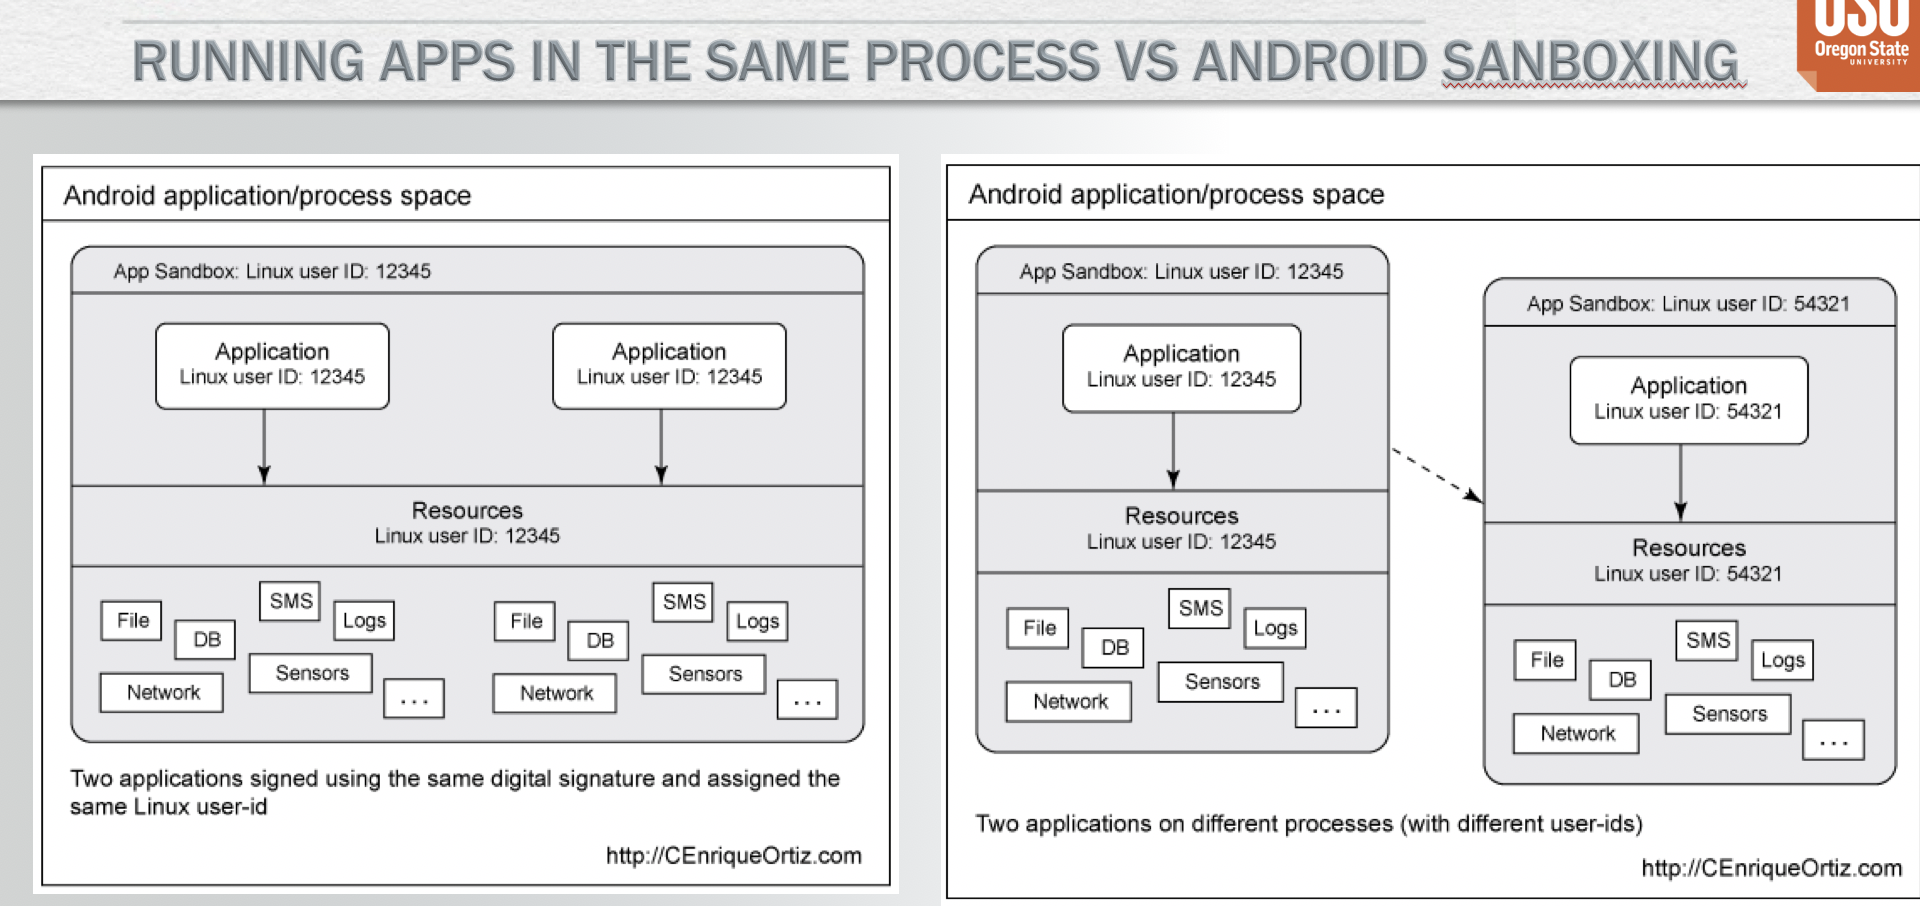
\includegraphics{P1.png}
\item System Security Bypasses – Jailbreaking, Rooting in Android, Security Enhancements
\item Mobile Malware Genesis, started in 2000-2004
\item Middle Ages – 2005-2006, 2006-2008
\item Calm Before the Storm – 2008-2010, New Platforms with Smartphone revolution, market share changed, new capabilities
\item Symbian Worm YXES: First Mobile Botnet
\item Ikee – first Ios malware. Jailbroken phones (2009)
\item First Android Malware in the wild. Fakeplayer, Tapsnake
\item Andrew Malware Revolution – exponential increase
\item Geimini – first android botnet – 2010, China, Leaks sensitive info to a remote server
\item PJApps – Interception of SMS messages, Found 2011 targeting Chinese users
\item Droiddream – android market nightmare, 2011, many apps, XOR obfuscation (embeded key), attempts to root device using two public exploits
\item Google Action – Remote Kill Switch
\item Android Fundamentals
 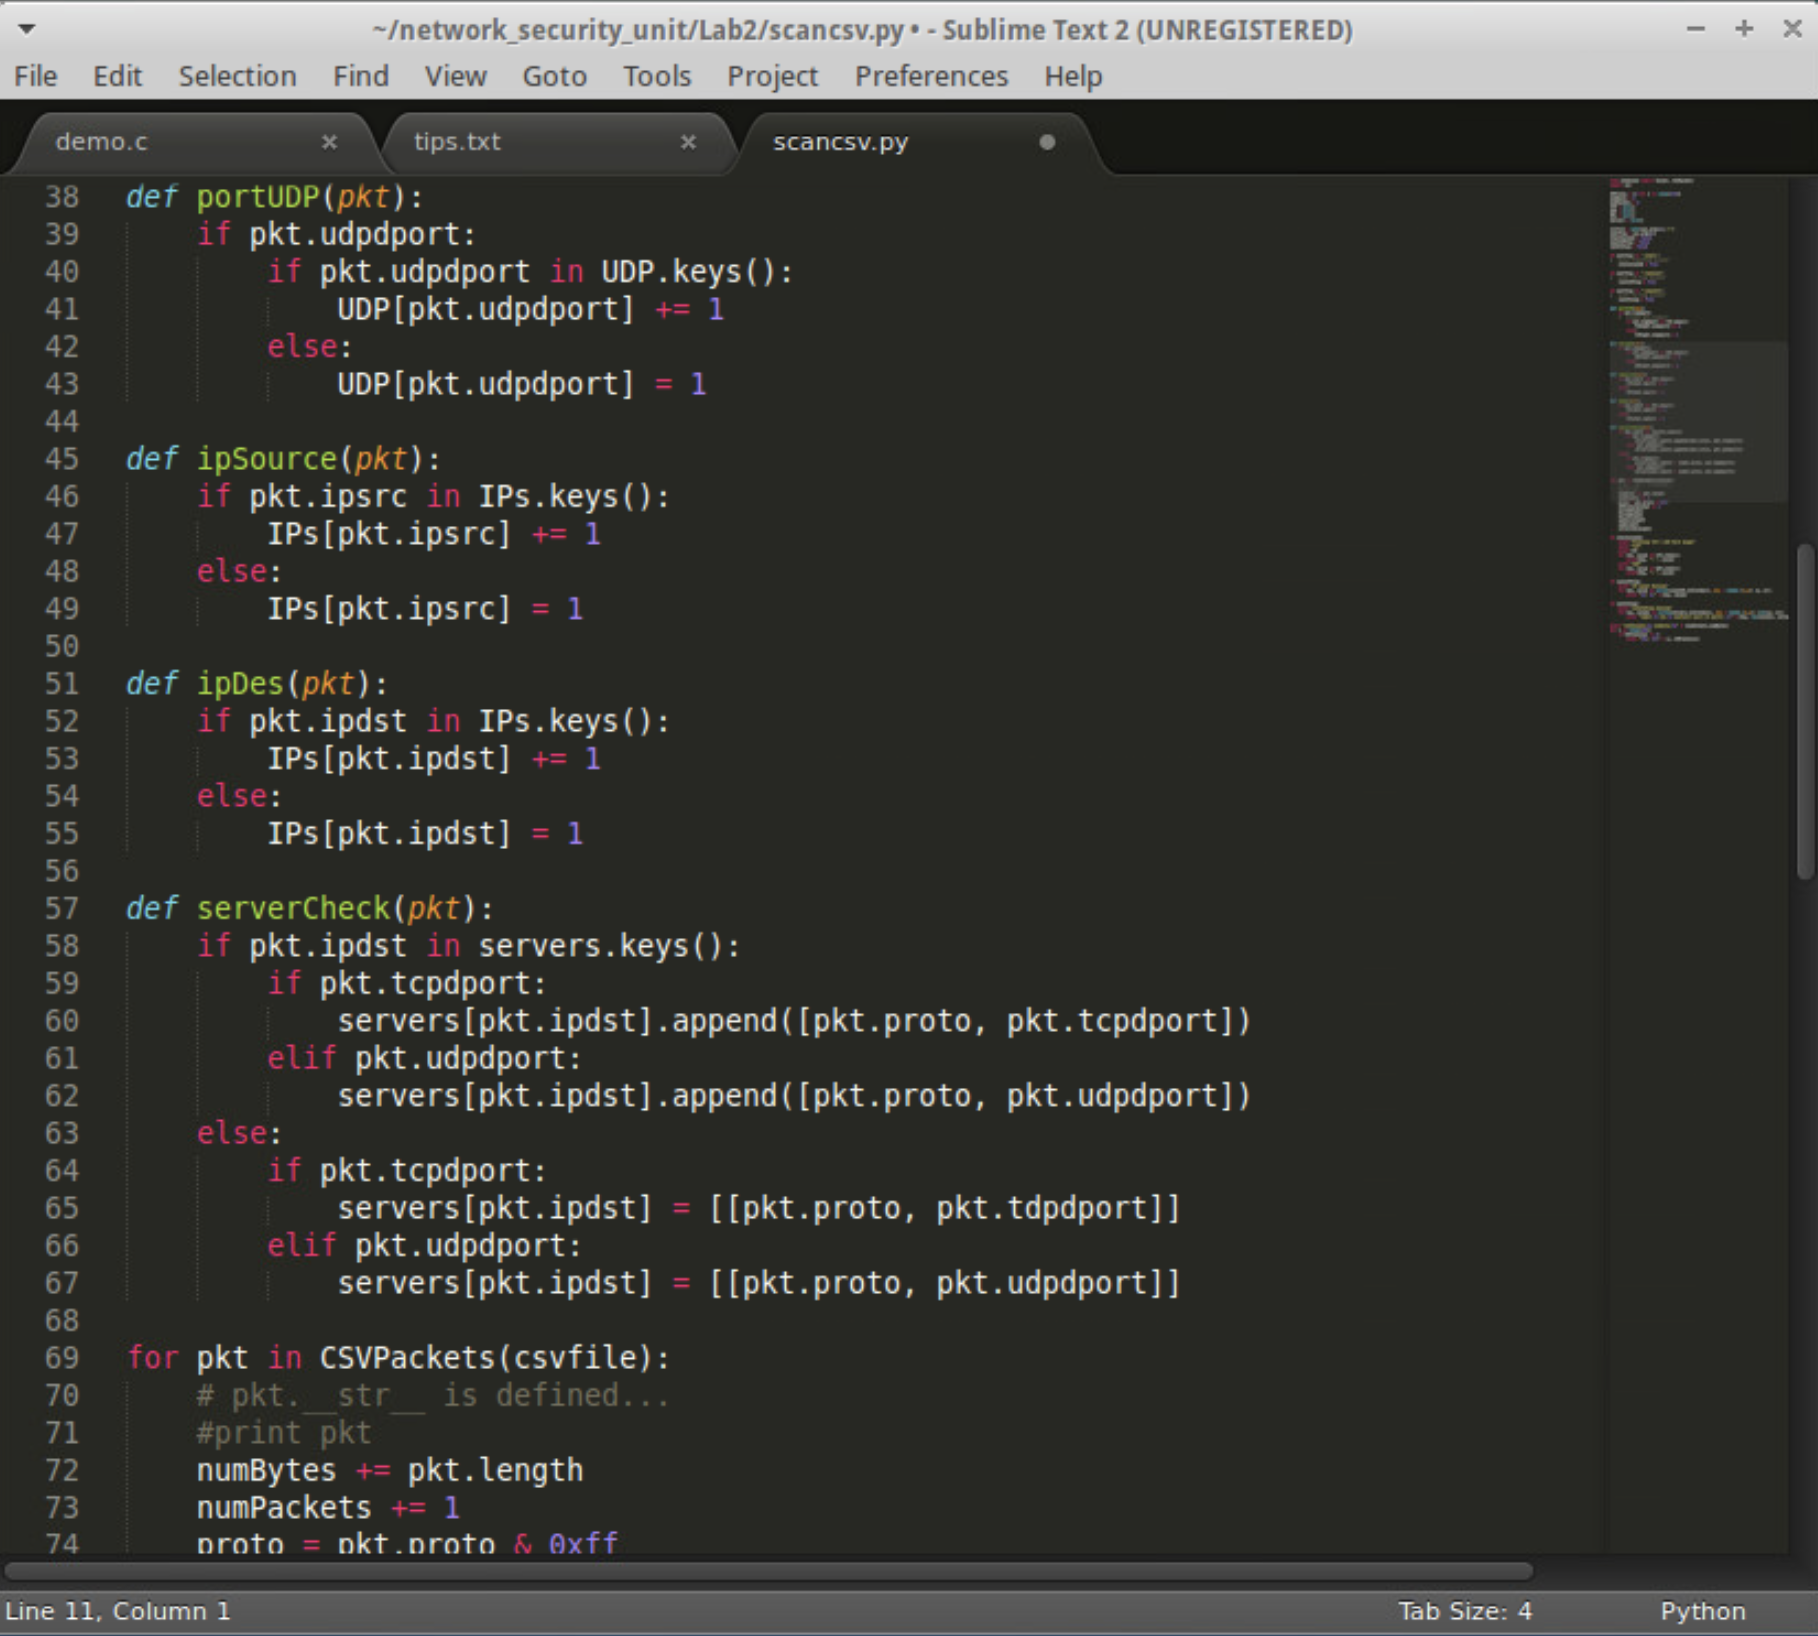
\includegraphics{P2.png}
\item Android Runtimes, Dalvik architectures
\item Application sandboxing in android vs linux
\item Android application components: Activities, Services, Broadcast Receivers, Content Providers
\item Android interprocess communication: official and nonofficial
\item Intents – messages between components
\item Sticky Broadcasts
\item Android application permissions
\item Android Manifest.xml encoded inside the APK file.
\item Labs and Slides related to the labs, tools
\item Appendix Slides
\item Analog Systems (1G), Digital Cellular Networks (2G), Mobile Broadband Data (2.5G-3G), IP Networks (3.5G & 4G)


\end{itemize}
% --------------------------------------------------------------
%     You don't have to mess with anything below this line.
% --------------------------------------------------------------
 
\end{document}
